\section{Hardware Components and Constructions}

.. generic description and diagram .. (Chris)

\subsection{VXS/VME crates and CPU units (Abbott)}

\subsection{Trigger Disctribution system modules (TS, TD. TI)(William)}
	
\subsection{Signal Distribution module (SD)(Cody)}

\subsection{Flash ADC module (FADC250)(Hai)}

\subsection{Discriminator Scaler module (DSC2)}

The Discriminator Scaler module (DSC2) Fig.~\ref{fig:dsc2_board} is a 16 channel general purpose discriminator and scaler module designed as a 6U VME card. It replaces an older design,improving on jitter, noise, crosstalk, and adding new features.

\begin{figure}[hbt]
	\centering
	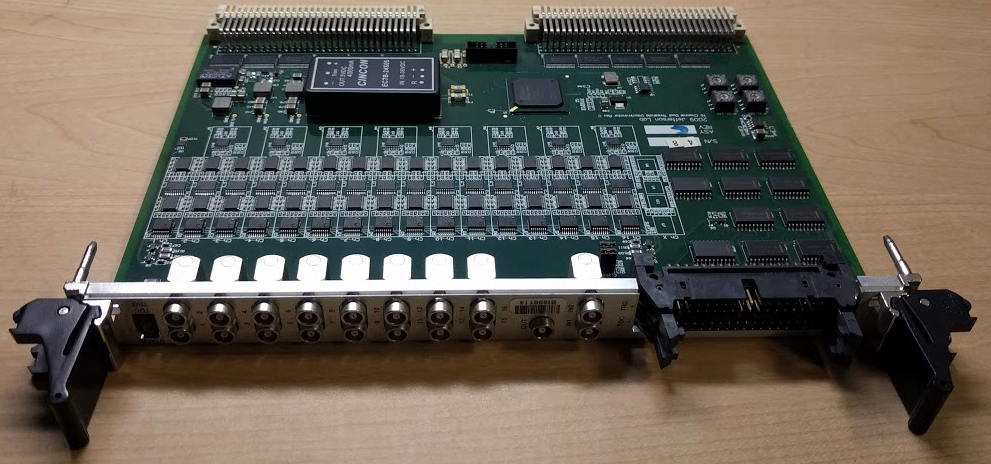
\includegraphics[width=1.0\columnwidth,keepaspectratio]{img/dsc2_board.png}
	\caption{Discriminator Scaler module (DSC2)}
	\label{fig:dsc2_board}
\end{figure}

\begin{center}
	DSC2 Specifications\\
	\begin{tabular}{| l | l |}
		\hline \hline
		Property			& Value				\\
		\hline
		{\bf Analog Discriminator}	&				\\
		Threshold			& 0 to -1023mV			\\
		Pulse width			& 4ns to 40ns			\\
		Dead-time			& 4ns typ. w/8ns pulser width	\\
		Maximum input rate		& $>$125MHz 			\\
		Ch-ch isolation			& $>$65dB			\\
		Threshold noise			& 1.3mV RMS typ.		\\
		Slew-rate delay disperson	& $<$20ps			\\
		Input-to-output delay		& $<$5ns			\\
		{\bf Digital Processing}	&				\\
		Digital delay step		& 4ns				\\
		Digital delay maximum		& 1us				\\
		Digital width maximum		& 1us				\\
		Maximum count rate		& 125MHz			\\
		\hline \hline
	\end{tabular}
\end{center}

\paragraph{Discriminator}
Inputs are single-ended LEMO and leading-edge discrimated by two different thresholds. Typically one threshold is used for time-to-digital applications and the other threshold is used for trigger applications. There are separate differential ECL outputs for each channel and threshold. Low jitter performance was an important goal of the design as this module will be used in high resolution applications. Fig.~\ref{fig:dsc2_jitter} shows the typical jitter as a function of a variety of input slew rate signals and threshold overdrive conditions.

\begin{figure}[hbt]
	\centering
	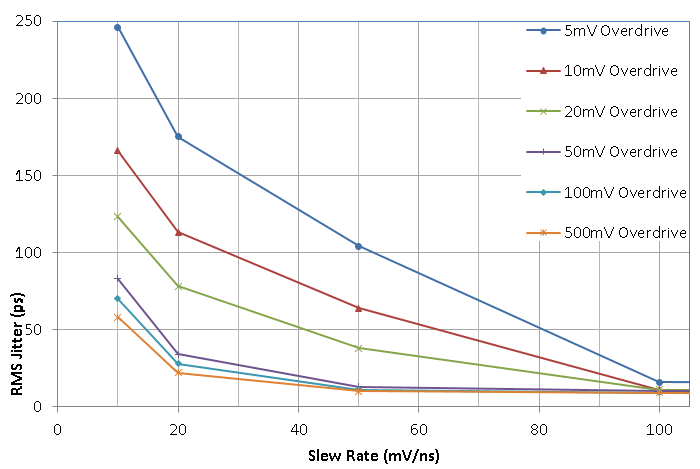
\includegraphics[width=1.0\columnwidth,keepaspectratio]{img/dsc2_jitter.png}
	\caption{Output Jitter vs Input slew rate and overdrive}
	\label{fig:dsc2_jitter}
\end{figure}

\paragraph{Digital Processing}
A Xilinx Spartan 3A FPGA is used to implement the VME interface, scalers, discriminator controls, and scaler event building features. Each channel and threshold has two scalers associated with it. The first scaler counts all threshold crossings for the input. The second scaler is gated using a front-panel input source, which can be useful to computing dead-time of channels and many other applications. Additionally, reference scalers are accumulated (a gated and ungated version) that count the elapsed time which can be used to normalize inputs scalers to Hz. All together there are 68 scalers, which can be slow to read over VME if using single-cycle transfers. An event builder is implemented that can synchronously read (and optionally clear) all scalers and build an event with this data. Over 100 events can be buffered and readout using the VME 2eSST protocol at 200MB/s.


\subsection{TDC modiles (v1190/v1290)(Sergey)}

\subsection{Drift Chamber Readout Board (DCRB)}

\begin{figure}[hbt]
	\centering
	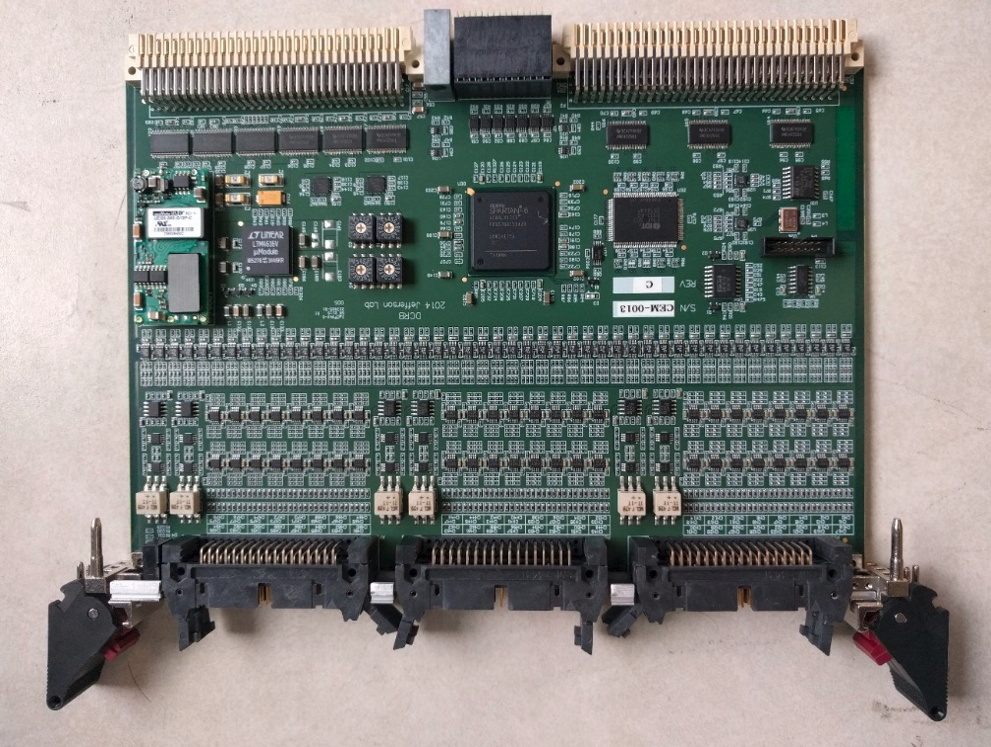
\includegraphics[width=1.0\columnwidth,keepaspectratio]{img/dcrb_board.png}
	\caption{Drift Chamber Readout Board (DCRB)}
	\label{fig:dcrb_board}
\end{figure}

The Drift Chamber Readout Board (DCRB) Fig.~\ref{fig:dcrb_board} is a 96 channel amplifier, discriminator, time-to-digital converter VXS module used to digitize and readout hits from the CLAS12 Drift Chambers. A single VXS crate of DCRB modules can readout a full region of the drift chambers for a single sector resulting in 18 VXS crates of DCRBs to instrument 6 sectors each having 3 regions of drift chamber.

\paragraph{Analog Inputs}
Each DCRB receives 96 differential analog signal pairs using twisted pair cabling from the drift chamber pre-amplifiers. The pre-amplfiers are located on the detector providing a gain of ~2.3mV/$\mu$A. On the DCRB each analog input channel is amplified by a voltage gain of 30 and then discriminated by a programmable threshold (common to all channels on the board with an effective chamber wire threshold range of 0 to 3.5/$\mu$A).

\paragraph{TDC Event Builder}
All discriminated channels go to a Xilinx Spartan 6 FPGA where a 96 channel 1ns resolution time-to-digital converter (TDC) is implemented in firmware. The TDC is based on the ISERDES2 shift register FPGA primitive that directly sample of the digital input with a single-data-rate (SDR) input register clocked at 1GHz. The TDC sampling clock is synchronized to the CLAS12 master oscillator making it easy to relate hit times in the drift chamber other detectors in CLAS12. TDC inputs are buffered supporting multiple hits allowing for an average hit rate of 4MHz per input before loss of data, which exceed the hits rates the chamber is designed for by a few orders of magnitude. Hits from groups of 16 channels are written into a large buffer that a linked-list content addressable memory (CAM) tracks for 16$\mu$s. When a L1A trigger signal is received a time window of hits is extracted from the TDC hit buffer. The readout time window times are supplied to the CAM, and the CAM provides the address of the last hit matching each readout time bin. The hit buffer is then read to extract the hit and also the address of the next hit in the buffer matching the time bin (this is the linked list behavior). The result is an extremely fast event builder with natural zero suppression that doesn't require time sorted data. Cleanup is accomplished by a timer that invalidates CAM entries after time bins are 16$\mu$s old. Hits for an event are assembled and buffered in a 2MByte external RAM which is readout through the VME bus using the 2eSST protocol at 200MB/s.

\paragraph{Calibration Support}
A programmable amplitude pulse generator is implemented that can inject test pulses directly to the DCRB differential amplifier inputs as well as to the pre-amplfiers that are on the detector. This provides a way to test points of failure, check channel gain, and check channel delays without any extra equipment. A scaler is implemented on each channel for slow control monitoring of all chamber wires.

\subsection{VXS Silicon Readout Module (VSCM)}
The CLAS12 Silicon Vertex Tracker (SVT) detector front-end utilizes the data driven FSSR2 ASIC for digitization. The VXS Silicon Readout Module (VSCM) Fig.~\ref{fig:vscm_board} was designed to interface the FSSR2 based front-end to the CLAS12 DAQ system. This system is capable of reading out all 33,792 SVT channels in 3 VXS crates.

\begin{figure}[hbt]
	\centering
	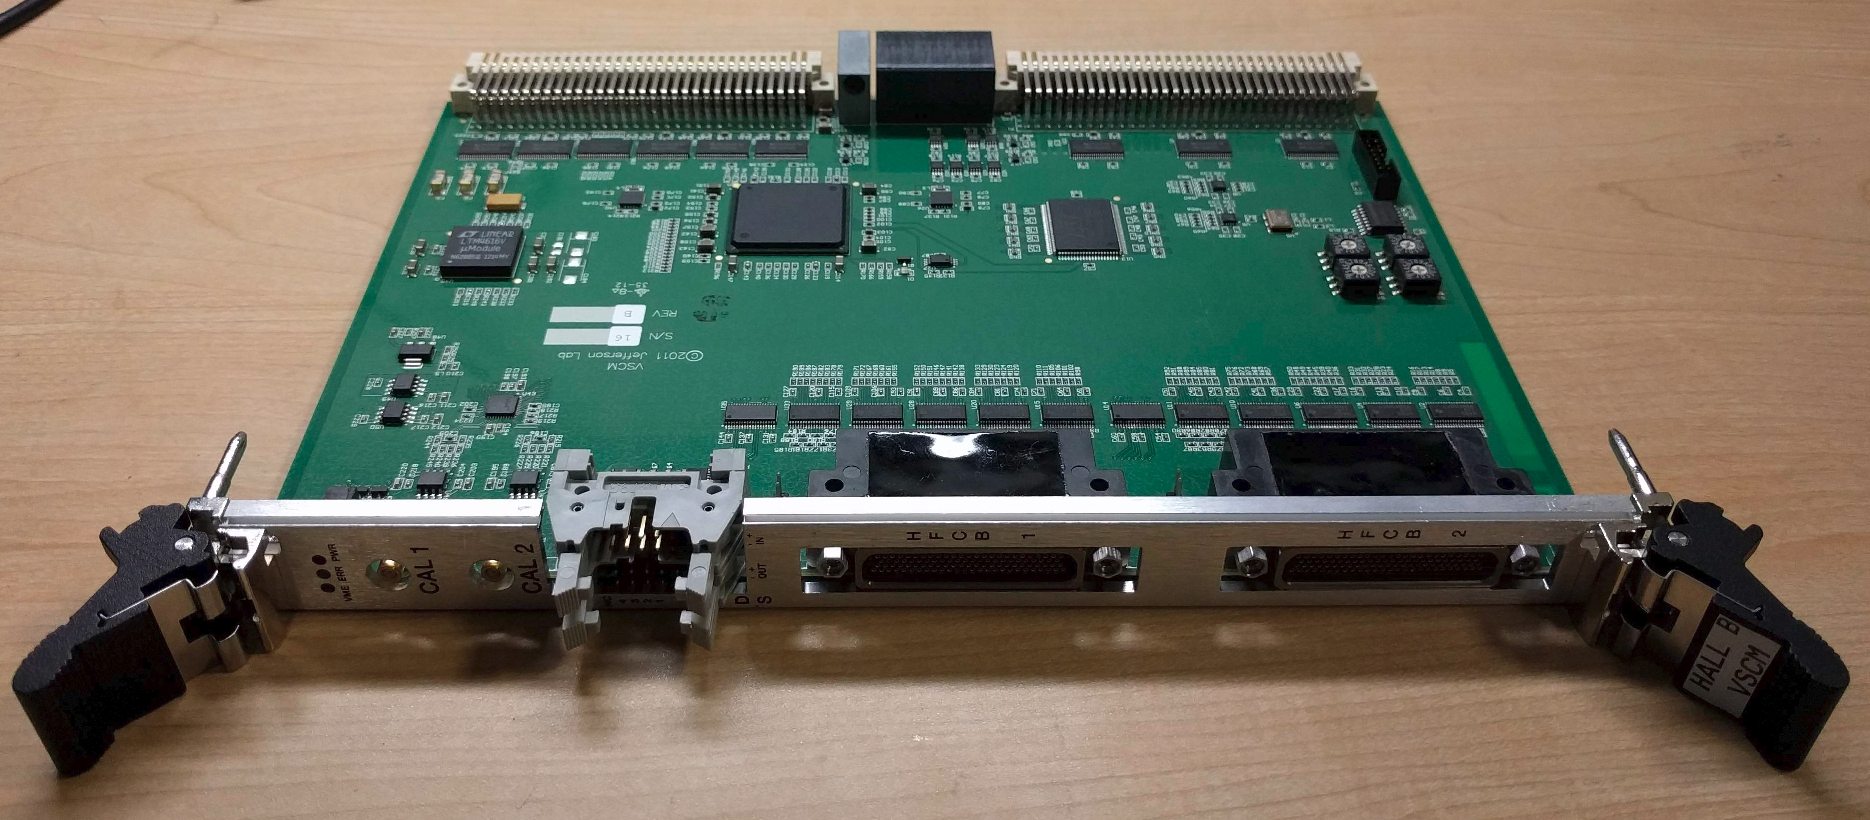
\includegraphics[width=1.0\columnwidth,keepaspectratio]{img/vscm_board.png}
	\caption{VXS Silicon Readout Module (VSCM)}
	\label{fig:vscm_board}
\end{figure}

The main features of the VSCM include:

\begin{itemize}
	\item Receives 8 FSSR2 streams, each at 840Mbps
	\item De-randomizes hits into an 8$\mu$s buffer
	\item 512k multi-hit, multi-event buffer
	\item Supports $>$1MHz trigger rate
	\item Programmable amplitude charge injector
	\item 1ns resolution time-to-digital converter (TDC)
	\item Per channel hit scaler
	\item FSSR2 synchronization, status, and control
\end{itemize}

\paragraph{Event Builder}
The VSCM deserializes the FSSR2 streams checking for errors and decoding the hits, which are stored in an 8$\mu$s circular memory. The hits are not guaranteed to be time ordered, so the timestamp and channel number are used to form the circular memory address (rather than storing in the order received). The VSCM also implements an 8 channel 1ns time-to-digital converter (TDC) which measures the logic OR of hits from each FSSR2 ASIC. This high time resolution is significantly better than the FSSR2 serial stream hit time resolution and is required for improved out-of-time hit rejection. The L1A trigger signal time is used to look back a fixed amount of time and extract a time window of hits from the circular memory, which correspond to the physics event. Non-zero hits are as assembled as an event and buffered in a 2MByte external RAM which is readout through the VME bus using the 2eSST protocol at 200MB/s.

The event data contains primarily two hit word types that together provide high time resolution and spatial hit resolution while keeping the front-end complexity low.

\begin{center}
	Low time resolution hit word\\
	\begin{tabular}{| l | l |}
		\hline \hline
		Property	& Description		\\
		\hline
		Hit Time	& 128ns resolution	\\
		Channel		& 0-1023 strip Id	\\
		Charge		& 0-7 threshold		\\
		\hline \hline
	\end{tabular}
\end{center}

\begin{center}
	High time resolution hit word\\
	\begin{tabular}{| l | l |}
		\hline \hline
		Property	& Description		\\
		\hline
		Hit Time	& 1ns resolution	\\
		Channel		& 0-7 chip Id		\\
		\hline \hline
	\end{tabular}
\end{center}

Fig.~\ref{fig:vscm_blockdiagram} shows the hardware block diagram of the module. Essentially a single low-cost Xilinx Spartan 6 FPGA was to implement the deserialization, buffering, event-building, monitoring, front-end configuration, time-to-digital conversion and monitoring.

\begin{figure}[hbt]
	\centering
	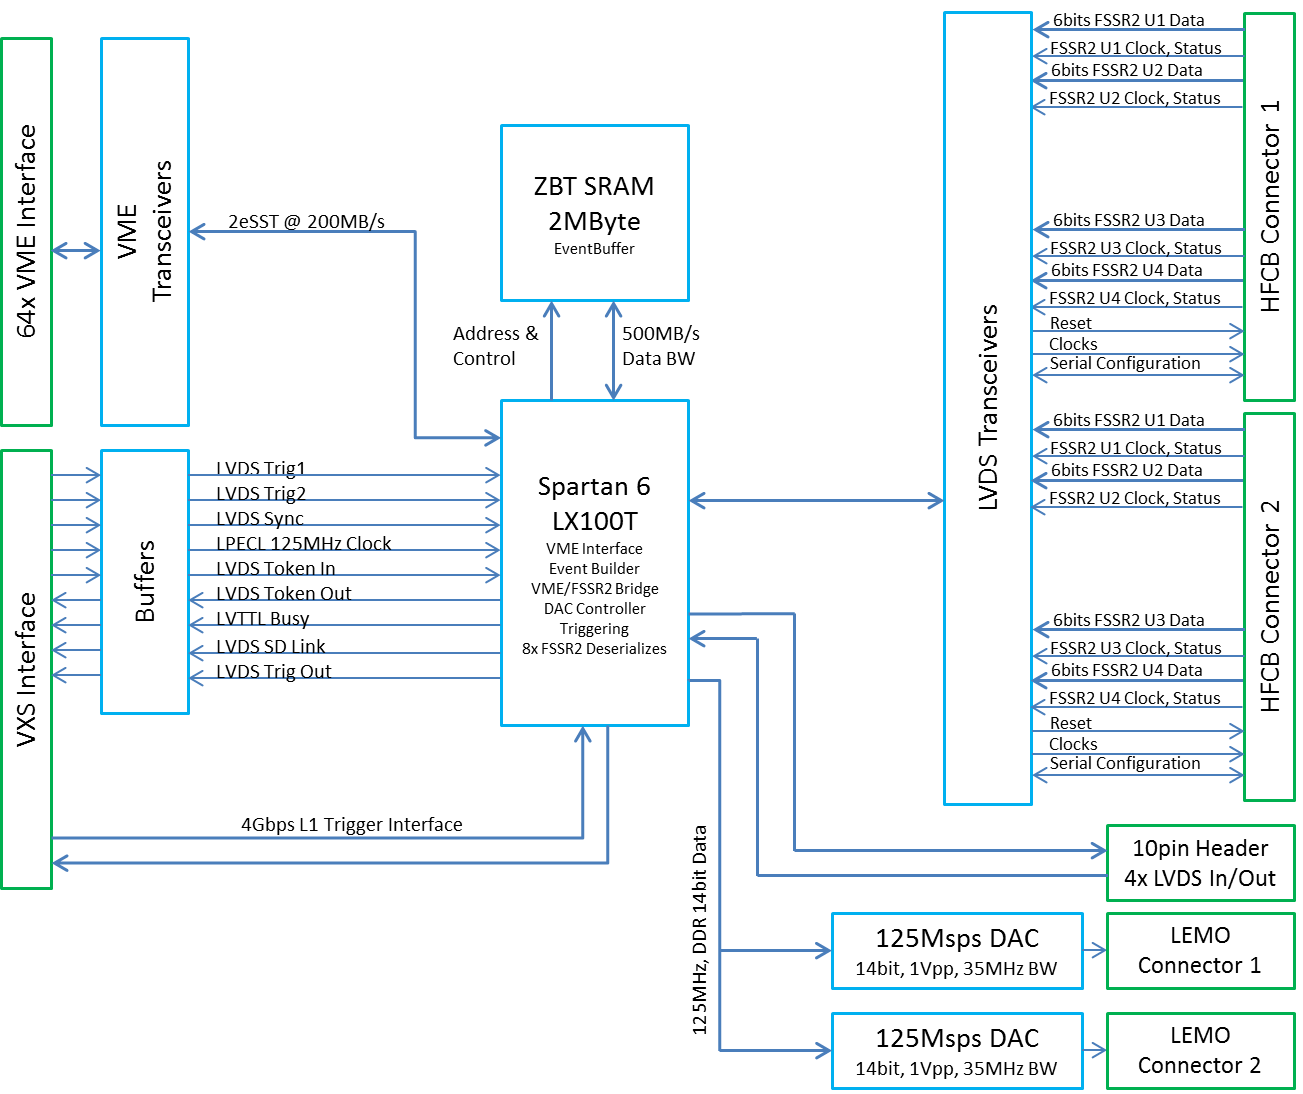
\includegraphics[width=1.0\columnwidth,keepaspectratio]{img/vscm_blockdiagram.png}
	\caption{VSCM Hardware Diagram}
	\label{fig:vscm_blockdiagram}
\end{figure}


\subsection{SSP board as fiber readout module(Ben)}
